%\documentclass[onecolumn]{article}

%define margins
%\usepackage[margin=1in,top=1.0in, left=1in,right=1in]{geometry}

%core packages
%\usepackage{siunitx} %for writing numbers with units vis \SI, \num
%\usepackage{amsmath} %for cases, multline environments
%\sisetup{detect-weight=true, detect-family=true}
%\usepackage{physics} %for \vqty, \dd, \dv
%\usepackage{graphicx} %for \includegraphics
%\usepackage{enumitem} %for indenting items in description environment
%\usepackage{caption}

%\usepackage[final]{changes} %for keeping track of edits
%\definechangesauthor[name={Matt Bovyn},color=blue]{MB}
%\definechangesauthor[name={Jun Allard},color=orange]{JA}

%for nicer Tau
%\usepackage{ upgreek }
%\renewcommand{\tau}{{\,\uptau}}

%citations with biblatex
%for S prefix, need input argument defernumbers=true
%then before \printbibliography need a \newrefcontext[labelprefix=S]
%\usepackage[backend=biber,defernumbers=true]{biblatex}
%\addbibresource{suppliment.bib}

%some citations from Mendelay don't play well with the default ascii encoding
%use utf8 instead
%\usepackage[utf8]{inputenc}    % utf8 support       %!!!!!!!!!!!!!!!!!!!!
%\usepackage[T1]{fontenc}       % code for pdf file  %!!!!!!!!!!!!!!!!!!!!

%to change the figure and table labels to S#
%\setcounter{table}{0}
%\renewcommand{\thetable}{S\arabic{table}}
%%\setcounter{figure}{0}
%\renewcommand{\thefigure}{S\arabic{figure}}

%\usepackage{authblk}

%bring in convenience commands
\input appendix1/preamble.tex

%\usepackage{hyperref}%for links, should always come last

%\begin{document}

%\title{Supplemental information for \\ Cargo navigation across 3D microtubule intersections}
%\date{}
%\author[a,1]{Jared Bergman}
%\author[b,c,1]{Matthew Bovyn}
%\author[d]{Manasa Gudheti}
%\author[b,c,e]{Steven Gross}
%\author[b,c,f,2]{Jun Allard}
%\author[a,g,h,2,3]{Michael Vershinin}
%\affil[a]{Department of Biology, University of Utah}
%\affil[b]{Department of Physics and Astronomy, University of California, Irvine}
%\affil[c]{Center for Complex Biological Systems, University of California, Irvine}
%\affil[d]{Visiting Scientist, Department of Biology, University of Utah}
%\affil[e]{Department of Developmental and Cell Biology, University of California, Irvine}
%\affil[f]{Department of Mathematics, University of California, Irvine}
%\affil[g]{Department of Physics and Astronomy, University of Utah}
%\affil[h]{Center for Cell and Genome Science, University of Utah}
%\affil[1]{JB and MB contributed equally to this work}
%\affil[2]{JA and MV contributed equally to this work}
%\affil[3]{To whom correspondence should be addressed. Email: vershinin\{at\}physics.utah.edu}

%\maketitle

%\newpage

%Contents: \\
%\begin{enumerate}[label=\arabic*,leftmargin=*,labelsep=2ex,ref=\arabic*]
%    \item[] Supplemental figures
%      \begin{enumerate}[label*=.\arabic*,leftmargin=*,labelsep=2ex]
%        \item[] Figure S1: Restoring force on BH \dotfill 3
%        \item[] Figure S2: Solutions to the heuristic model for ToW probability \dotfill 4
%        \item[] Figure S3: ToW times \dotfill 5
%        \item[] Figure S4: Mean motors engaged during ToW \dotfill 6
%      \end{enumerate}
%    \item[] Mathematical model of cargo dynamics
%      \begin{enumerate}[label*=.\arabic*,leftmargin=*,labelsep=2ex]
%        \item[] 1 Model description \dotfill 7
%        \item[] 2 Numerical simulation of the model \dotfill 11
%        \item[] 3 Model Results \dotfill 15
%      \end{enumerate}
%     \item[] Captions for supplemental movies \dotfill 22
%     \item[] Supplemental references \dotfill 23
%\end{enumerate}

%\newpage


\chapter{Mathematical Model for Routing at Intersections} \label{sec:model}

\begin{figure}
\centering
\includegraphics[width=4in]{appendix1/FvsL}
\caption[Restoring force on Bead Handles]{Restoring force on a glass bead (index of refraction 1.55, \SI{1000}{\nano\meter} radius) exerted by the HOT for various displacements from trap center. Calculations were performed using previously published software\cite{Nahmias2002}.}
\label{fig:BHforce}
\end{figure}

\clearpage

\begin{figure}
\centering
\includegraphics[width=12cm]{appendix1/heuristicEXP.pdf}
\caption[Solutions to the heuristic model for ToW probability]{Solutions to the heuristic model for ToW probability \\
A heuristic model (given in equation \ref{eq:rate_war}) poses the probability of undergoing ToW as the the probability of the cargo binding (with constant binding rate) to the crossing MT before leaving the ToW zone (see equation \ref{eq:ToW_zone} and figure \ref{fig:heuristic}). 
%Solutions to the model reproduce qualitative features of the simulated ToW probability for \SI{.5}{\micro\meter} and \SI{1}{\micro\meter} separation distances, shown in main text figure 4. The fact that the heuristic model does not qualitatively reproduce ToW probabilities for \SI{0}{\micro\meter} geometries highlights the importance of steric effects at these geometries. 
Solutions shown as solid curves. Bars represent 95\% confidence intervals for corresponding experimental data. Bars for data at \SI{.5}{\micro\meter} shifted slightly to aid the eye. Solutions plotted with $\kon^\text{macro}$ set to \SI{1}{\per\second}.
} \label{fig:heuristicEXP}
\end{figure}

\clearpage

\begin{figure}
\centering
\includegraphics[width=6in]{appendix1/ToWtime_fits.pdf}
\caption[Empirical cumulative probability distributions for ToW times]{Empirical cumulative probability distributions for ToW times \\
The time for which cargos underwent ToW in 90 degree (normal) geometries was measured in experiments and simulations. Cumulative distributions are shown for each geometry. To aid interpretation, medians are highlighted with dotted lines. Fits to gamma cumulative distribution functions are shown in dashed lines. Good fits to gamma distributions with shape parameter 2-3 indicate distributions are well approximated as generated from 2-3 independent exponential events which we interpret as motor unbinding events.
} \label{fig:ToWtimes}
\end{figure}

\clearpage

\begin{figure}
\centering
\includegraphics[width=4in]{appendix1/num_engagedEXP.pdf}
\caption[Number of motors engaged on MTs during ToW]{ Number of motors engaged on MTs during ToW\\
The mean number of motors engaged on the primary (\textit{top}) and crossing (\textit{center}) MTs during simulated ToWs are shown for each geometry. Additionally, the ratio of the mean number of motors engaged on the crossing MT to the mean number engaged on the primary MT is shown (\textit{bottom}). Data are represented as mean +/- SEM. Separation distances are colored as specified in the legend in the top panel.
} \label{fig:num_engagedEXP}
\end{figure}

\clearpage

%\vspace*{2\baselineskip}
%\centerline{\textbf{\LARGE Mathematical model of cargo dynamics}}
%\vspace{4\baselineskip}

%%%%%%%%%%%%%%%%%%%%%%%%%%%%%%%%%%%%%%%%%%%%%%%%%
\section{Model description} \label{description}

We present a three dimensional mesoscale model for the dynamics of the cargo, which takes into account rotational and translational diffusion, as well as stochastic stepping and binding of the motors. The locations of the cargo bead and motors attached to it are governed by a set of stochastic ordinary differential equations. Binding state and location of the motor head along the microtubule (MT) are considered discrete states and transitions between them occur stochastically, modeled as Poisson processes. We construct a Monte Carlo numerical simulator, based on a hybrid Euler-Maruyama-Gillespie scheme, and simulate an ensemble of stochastic trajectories, from which we  derive probabilities for tug of war and switching.

Motors in the model have two states:
\begin{description}[labelindent=\parindent,font=\normalfont]
\item[Bound:] A motor $i$ is defined by two points: one represents the the motor domains, which we call the head $\vec{h}^i$; the other represents the location at which the motor is bound to the bead, which we call the anchor $\vec{a}^i$. The motor has a rate of stepping along the MT $\kstep^i$ and a rate of unbinding from the MT $\koff^i$.
\item[Unbound:] A motor $i$ is defined by one point, the anchor location $\vec{a}^i$. The motor has a rate of binding to MT $j$, $\kon^{i,j}$, that depends on its location relative to the MT as described below.
\end{description}
We track the anchor locations, head locations of bound motors, the location of the cargo center $\vec{c}$, and the cargo orientation $\vec{\theta}$.

%**************************************************************************************************************
\subsection{Stochastic ordinary differential equations for cargo motion}

\begin{figure}
\centering
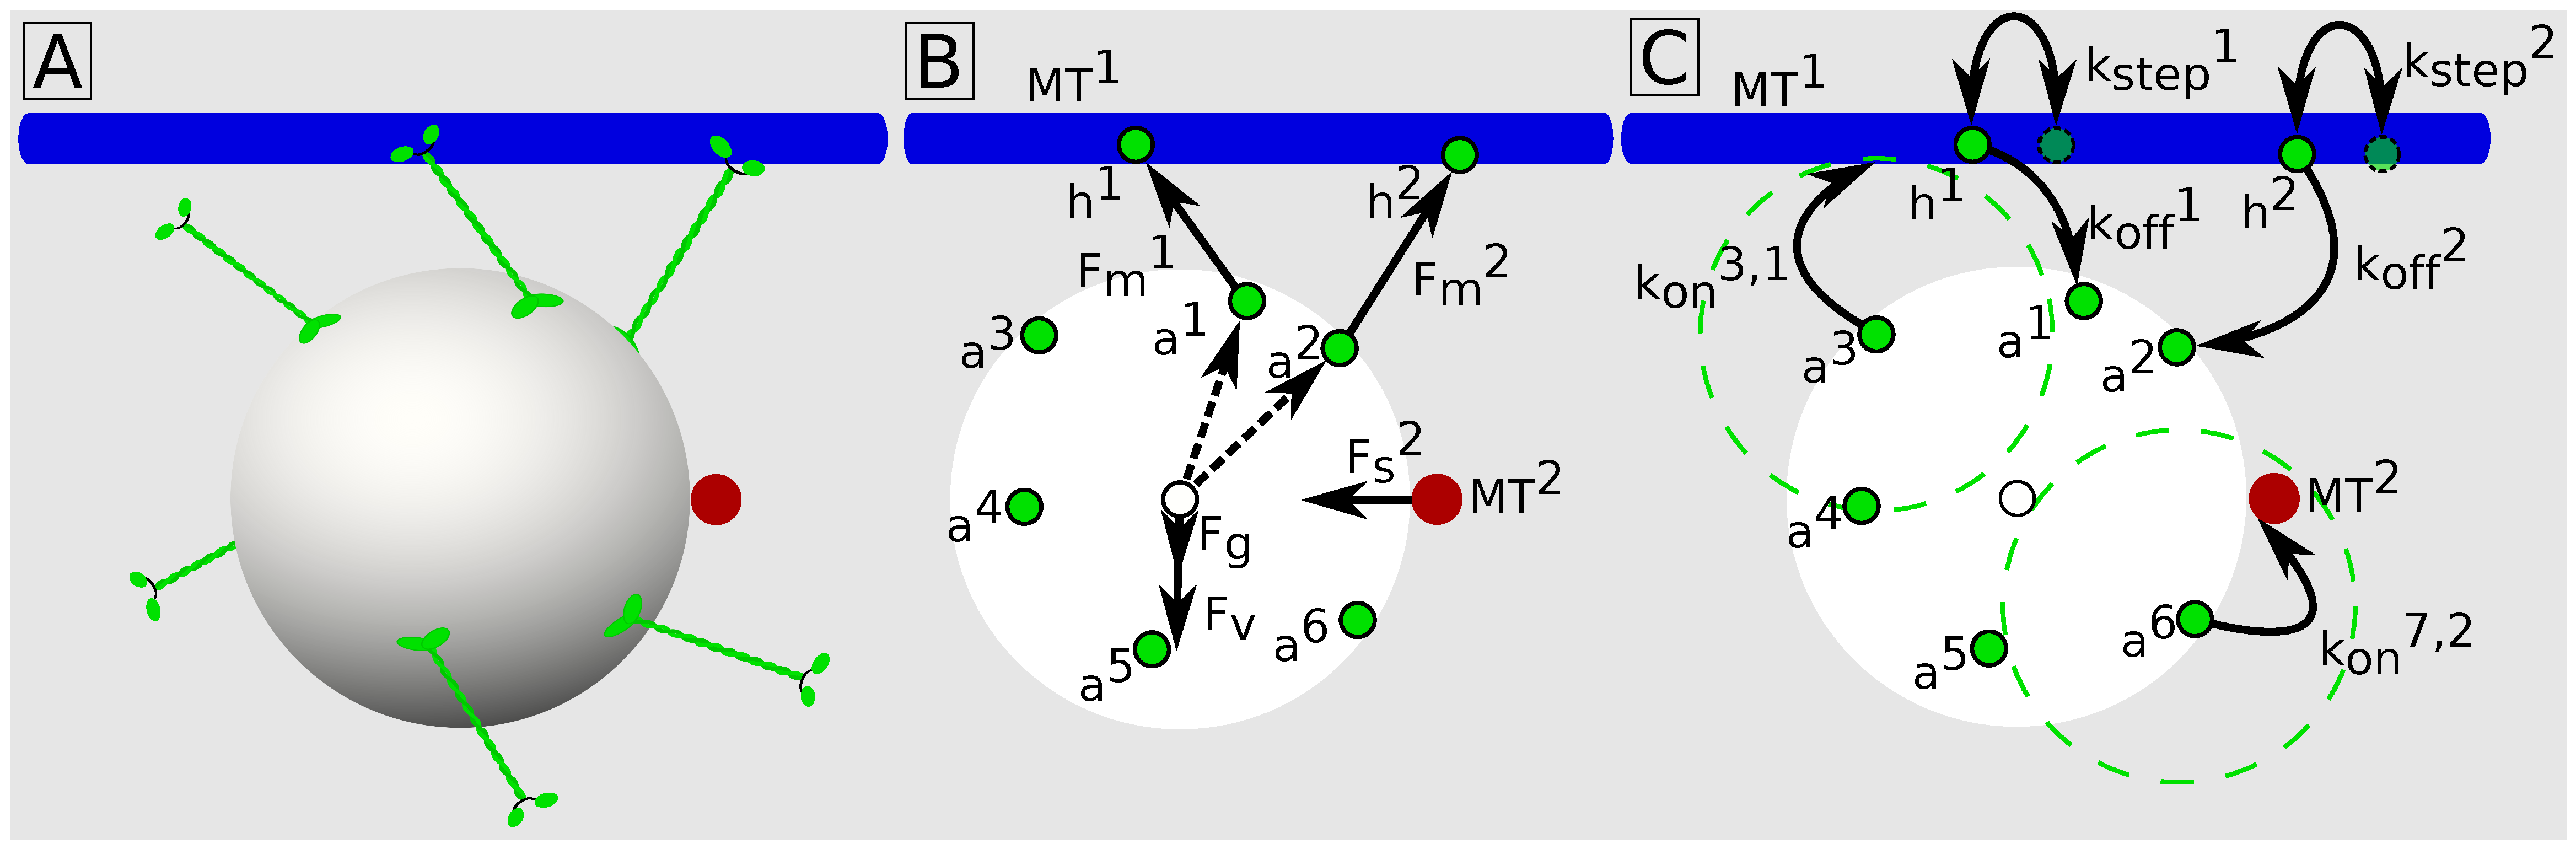
\includegraphics[width=6.5in]{appendix1/diagrams.eps}
\caption[Diagrams of simulated cargo dynamics]{Diagrams of cargo dynamics \\
A) Schematic of a model cargo in motion. Kinesin motors are shown in green, primary MT in red, crossing MT in blue, and bead in white. \\
B) Free body diagram of the cargo corresponding to the cartoon in A. Anchor locations $\vec{a}^i$ and head locations $\vec{h}^i$ are shown with green dots. Cargo center location $\vec{c}$ is shown with a white dot with black outline. Forces are shown with solid arrows. Dashed arrows show the lever arm through which the motor forces exert torque. \\
C) Diagram showing the possible state changes corresponding to the cartoon in A. Unbound motors have on rates greater than 0 if their anchor is less than 1 motor length from a MT. Bound motors have rates of stepping and unbinding.
} \label{fig:FBD}
\end{figure}

We first impose force-balance on the cargo. The motion of the cargo is the inertialess regime (Reynolds number $\sim 10^{-6}$), so we omit the inertia term. A free body diagram showing the deterministic forces acting on model cargo is shown in figure \ref{fig:FBD}B. All forces must balance, so
\begin{equation} \label{eq:forcebalance}
\sum \vec{F} = \underbrace{\sum_i \vec{F}_m^i}_{\text{motor forces}} + \underbrace{\sum_j \vec{F}_s^j}_{\text{steric forces}} + \underbrace{\vec{F}_g}_{\text{force of gravity}} + \underbrace{\vec{F}_b}_{\text{Brownian force}} + \underbrace{\vec{F}_v}_{\text{viscous force}} = 0.
\end{equation}
Similarly, we can write the balance of torques on the model cargo
\begin{equation} \label{eq:torquebalance}
\sum \vec{\tau} = \underbrace{\sum_i \vec{\tau}_m^i}_{\text{torque from motor forces}} +\underbrace{\vec{\tau}_b}_{\text{Brownian torque}} + \underbrace{\vec{\tau}_v}_{\text{viscous torque}} = 0.
\end{equation}
By specifying the forms of each of these forces below, we construct the equations of motion of the cargo center $\vec{c}$ and cargo orientation $\vec{\theta}$.

%------------------------------------------------------------------------------------------------------------------------------
\subsubsection*{Motor forces}

We model the force that the motor exerts on the cargo as originating from the stretch in spring-like motor stalks, based on experimental measurements \cite{Kojima1997,Jeney2004} and in line with  previous models \cite{Erickson2011,Korn2009,Kunwar2008}. The form of this force is that of a one-way (tension-only) spring with rest length equal to the length of the motor. The force $\vec{F}_m^i$ exerted by motor $i$ on the cargo bead is given by
\begin{equation} \label{eq:motor_spring}
\vec{F}_m^i \left( \vec{a}^i,\vec{h}^i \right) = 
\begin{cases}
	- \kappa_m \left( \left| \vec{h}^i - \vec{a}^i \right| - L \right) \left( \frac{\vec{h}^i - \vec{a}^i}{\left| 		\vec{h}^i - \vec{a}^i \right|} \right) & \left| \vec{h}^i - \vec{a}^i \right| >  L\\
	0 & \text{otherwise}
\end{cases}.
\end{equation}
This force also exerts a torque on the cargo bead, given by the cross product of the lever arm and force vector
\begin{equation} \label{eq:motor_torque}
\vec{\tau}_m^i \left( \vec{a}^i,\vec{h}^i,\vec{c} \right)= 
\left( \vec{a}^i - \vec{c} \right) \times \vec{F}_m^i \left( \vec{a}^i,\vec{h}^i \right).
\end{equation}

%------------------------------------------------------------------------------------------------------------------------------
\subsubsection*{Steric forces}


The cargo bead and MTs are prevented from overlapping in space by a steric force with the form of a one-way (compression-only) spring, given for MT $j$ by 

\begin{equation} \label{eq:steric_force}
\vec{F}_s^j(\vec{c})= 
\begin{cases}

	- \kappa_s \left(R - \vqty\Big{ \rvec{\vec{c}} } \right) \left( \frac{\rvec{\vec{c}}}{\vqty\big{ \rvec{\vec{c}} }} \right) & \vqty\Big{ \rvec{\vec{c}} } <  R\\
	
	0 & \text{otherwise}
	
\end{cases},
\end{equation}
where $\rvec{\vec{p}}$ is a vector from point $\vec{p}$ to the nearest point on the MT. This is found by computing the perpendicular distance from $\vec{p}$ to the MT surface, given by
%formula for vector from point to center of MT
\def\ceq{\left( \xmt^j-\vec{p} \right) - \left( \left( \xmt^j - \vec{p} \right) \cdot \dmt^j \right) \dmt^j}
%shortcut for R_MT/ceq because I want the parentheses to be the same size
\def\rbyceq{\frac{R_\text{MT}}{\vqty\bigg{\ceq}}}
%
\begin{multline} \label{eq:r_vec}
\rvec{\vec{p}} = 
\left( 1- \rbyceq \right)  \\
\left( \ceq \vphantom{\rbyceq} \right).
\end{multline}

%------------------------------------------------------------------------------------------------------------------------------
\subsubsection*{Force of gravity}

The experimental system uses a silica bead with density greater than water as the cargo. Therefore the model cargo experiences a small but significant force due to gravity given by the buoyancy of the bead,
\begin{equation} \label{eq:F_g}
\vec{F}_g= \frac{4}{3} \pi R^3 (\rho_b - \rho_w) \vec{g},
\end{equation}
where $\rho_b$ and $\rho_w$ are the mass densities of the silica bead and water, respectively.

%------------------------------------------------------------------------------------------------------------------------------
\subsubsection*{Brownian force}

The Brownian force $\vec{F}_b$ is a random variable with mean 0 and variance $2 k_B T \xi$, where $\xi$ is the drag coefficient and $k_B T$ is the thermal energy unit. Specifically,
\begin{align} \label{eq:Brownian_force}
\ev{\vec{F}_b} &= \vec{0} \\
\ev{\vec{F}_b(t) \cdot \vec{F}_b(s)} &= 2 (k_B T) (6 \pi \eta R) \delta(t-s)
\end{align}
where we have inserted the translational drag coefficient of a sphere at low Reynold's number and $\delta(x)$ is the Dirac delta function.

Similarly, the Brownian torque on the bead is a random variable characterized by
\begin{align} \label{eq:Brownian_torque}
\ev{\vec{\tau}_b} &= \vec{0} \\
\ev{\vec{\tau}_b(t) \cdot \vec{\tau}_b(s)} &= 2 (k_B T)(8 \pi \eta R^3) \delta(t-s).
\end{align}

%------------------------------------------------------------------------------------------------------------------------------
\subsubsection*{Viscous force}

In the low Reynolds  limit, linear drag dominates. The drag on the cargo is thus given by Stokes' Law,
\begin{equation} \label{eq:trans_drag}
\vec{F}_v=-6 \pi \eta R \dv{\vec{c}(t)}{t}.
\end{equation}
The viscous torque is given by the rotational analogue to Stokes' Law,
\begin{equation} \label{eq:rot_drag}
\vec{\tau}_v=-8 \pi \eta R^3 \dv{\vec{\theta}(t)}{t}.
\end{equation}

%------------------------------------------------------------------------------------------------------------------------------
\subsubsection*{Construction and discretization of the stochastic ordinary differential equations}

With the forms of forces known, we  rewrite equations \ref{eq:forcebalance} and \ref{eq:torquebalance} as a pair of coupled ordinary stochastic differential equations
\begin{equation} \label{eq:cSDE}
\dv{\vec{c}(t)}{t} = 
%
\frac{1}{6 \pi \eta R} \left( 
\sum_i \vec{F}_m^i \left( \vec{a}^i(t) ,\vec{h}^i(t) \right) + 
\sum_j \vec{F}_s^j(\vec{c}(t)) + 
\vec{F}_g 
\right) + 
%
\frac{1}{6 \pi \eta R} \vec{F}_b(t)
\end{equation}
and
\begin{equation} \label{eq:thetaSDE}
\dv{\vec{\theta}(t)}{t}=
%
\frac{1}{8 \pi \eta R^3} \left( 
\sum_i \vec{\tau}_m^i \left( \vec{a}^i(t) ,\vec{h}^i(t) ,\vec{c}(t) \right) 
\right) + 
%
\frac{1}{8 \pi \eta R^3} \vec{\tau}_b(t),
\end{equation}
Equation \ref{eq:cSDE} is a specific implementation of the overdamped Langevin equation, used in Brownian dynamics. Equation \ref{eq:thetaSDE} is its rotational counterpart.

We discretize these equations according to the Euler-Maruyama method. For an update from the $n$th timestep at time $t_n$ to the next time $t_{n+1}$ with $\Delta t \equiv t_{n+1}-t_n$, the discretization is
\begin{multline} \label{eq:cSDE_discretized}
\vec{c}(t_{n+1}) = \vec{c}(t_n) +
\frac{1}{6 \pi \eta R} \left( \sum_i \vec{F}_m^i \left( \vec{a}^i(t_n) ,\vec{h}^i(t_n) \right) + \sum_j \vec{F}_s^j(\vec{c}(t_n)) + \vec{F}_g \right) \Delta t \\
+ \sqrt{2 \frac{k_B T}{6 \pi \eta R} \Delta t} \;\vec{G}_c(t_n)
\end{multline}
and
\begin{equation} \label{eq:thetaSDE_discretized}
\vec{\theta}(t_{n+1})= \vec{\theta}(t_n) +
\frac{1}{8 \pi \eta R^3} \left( \sum_i \vec{\tau}_m^i \left( \vec{a}^i(t_n) ,\vec{h}^i(t_n) , \vec{c}(t_n) \right) \right) \Delta t + \\
\sqrt{2 \frac{k_B T}{8 \pi \eta R^3} \Delta t} \;\vec{G}_\theta(t_n).
\end{equation}
%where $\vec{G}_c^n = \begin{pmatrix} G_1^n \\ G_2^n \\ G_3^n \end{pmatrix}$ is vector of three independent gaussian random variables with mean \num{0} and variance \num{1}, characterized by $\expval{G_\alpha(n) G_\beta(n')} = \delta^{\alpha\beta} \delta^{n n'}$, with $\alpha$ and $\beta$ denoting any pair of cartesian coordinates and $n$ and $n'$ denoting any pair of time steps
where $\vec{G}_c^n$ and $\vec{G}_\theta^n$ are two mutually uncorrelated vectors of three independently and identically distributed gaussian random variables with mean \num{0} and variance \num{1}.

%------------------------------------------------------------------------------------------------------------------------------
\subsubsection*{Update of anchor locations}

Since the motors are statically bound to the bead, the change in their locations is fully defined by the change in the location of the center of the bead $\vec{c}(t_{n+1})-\vec{c}(t_n)$ and the change in the orientation of the bead $\vec{\theta}(t_{n+1}) - \vec{\theta}(t_n)$.

The change in the bead orientation $\vec{\theta}(t_{n+1}) - \vec{\theta}(t_n)$ corresponds to a vector pointed along the axis of rotation of the bead with a length corresponding to the magnitude of the rotation in radians. This vector can be converted into a rotation matrix $\mathbf{M}_R(t_n)$. The next location of anchor $i$ is then calculated by finding
\begin{equation} \label{eq:anchor_update}
\vec{a}^i(t_{n+1})=\vec{a}^i(t_n) + \left( \vec{c}(t_{n+1})-\vec{c}(t_n) \right) + 
\left( \mathbf{M}_R(t_n) \left( \vec{a}^i(t_n) - \vec{c}(t_n) \right) + \vec{c}(t_n) \right).
\end{equation}

%**************************************************************************************************************
\subsection{Poisson processes}


We model all state transitions in the system as Poisson processes, diagrammed in figure \ref{fig:FBD}C. Experiments have reported exponential distributions of times between steps \cite{Carter2005} and times before unbinding \cite{Kunwar2011}. This is also the most basic assumption we can make for times before binding.

%\begin{figure}
%\centerline{\includegraphics[width=5cm]{CTMC.jpg}}
%\caption{Continuous time Markov chain diagram} \label{fig:CTMC}
%\end{figure}

%------------------------------------------------------------------------------------------------------------------------------
\subsubsection*{Stepping}

Kinesin motors step processively along MT tracks in a hand-over-hand fashion, with each motor domain taking \SI{16}{\nano\meter} steps \cite{Yildiz2004} that move the center of mass of the motor forward by \SI{8}{\nano\meter} \cite{Svoboda1993}. The rate at which the motor steps, and thus the motor velocity, depends on the load the motor is stepping against in a way well modeled as 
\begin{equation} \label{eq:stepping}
\kstep^i = 
\begin{cases}
\frac{v}{d}\left(1-F_m^i/F_s \right)^w & F_m^i < F_s \\
0 & F_m^i \geq F_s
\end{cases},
\end{equation}
as described in \cite{Kunwar2010}.

When a motor steps, it is moved forward along the direction of the MT $j$ to which it is bound by the step distance $d$. This translates to an update of the head position 
\begin{equation} \label{eq:step_head}
\vec{h}^i(t_{n+1}) = \vec{h}^i(t_n) + d \left(\dmt^j \right).
\end{equation}

%------------------------------------------------------------------------------------------------------------------------------
\subsubsection*{Unbinding}

Kinesin unbinds from the MT with a rate dependent on the force experienced by the motor. Measurements have shown that unbinding rate increases exponentially below stall \cite{Milic2014}. Above stall, measurements have shown that unbinding rate increases only slowly with increasing force \cite{Kunwar2011}. Therefore, we state the unbinding rate as
\begin{equation} \label{eq:unbinding}
\koff^i = 
\begin{cases}
\epsilon_0 \exp(F_m^i/F_d) & F_m^i \leq F_s \\
a+b F_m^i & F_m^i>F_s
\end{cases}.
\end{equation}
When a motor unbinds, it is simply put into the unbound state as defined at the beginning of this section.

%------------------------------------------------------------------------------------------------------------------------------
\subsubsection*{Binding}

The conditions which govern the rate of binding to the MT are not well known. In the absence of detailed experimental elucidation, we make only the most basic assumptions possible: the motor domains must be able to reach the MT to bind, and, if this condition is met, the motor binds with a constant rate. This translates to an on rate for motor $i$ to MT $j$ given by
\begin{equation} \label{eq:binding}
\kon^{i,j} = 
\begin{cases}
\pi_0^{\text{micro}} & \abs{ \rvec{\vec{a}^i} } \leq L\\
0 & \text{otherwise}
\end{cases}
\end{equation}
where $\rvec{\vec{a}^i}$ is given by equation \ref{eq:r_vec}.

When a motor $i$ binds to MT $j$, the head location is placed at the location on the MT nearest the anchor location $\vec{a}^i$, given by 
\begin{equation} \label{eq:bind_head}
\vec{h}^i(t_{n+1})=\vec{a}^i(t_n) + \rvec{\vec{a}^i(t_n)}.
\end{equation}

%%%%%%%%%%%%%%%%%%%%%%%%%%%%%%%%%%%%%%%%%%%%%%%%%
\section{Numerical simulation of the model} \label{sec:simulation}

Section \ref{description} outlines a numerical scheme for updating for the model's dynamic variables in equations \ref{eq:cSDE_discretized}, \ref{eq:thetaSDE_discretized} and \ref{eq:anchor_update} over a timestep $\Delta t$. We simulate the model forward in time using these equations. Time steps are chosen dynamically. The largest stable time step for the Euler-Maruyama scheme is given by $\xi/\kappa$, where $\xi$ is the drag coefficient and $\kappa$ is the spring constant of the stiffest operating spring. The maximum time step is chosen based on the springs active during that step. The equivalent stiffness of multiple active motor springs is taken into account, but the steric spring in equation~\ref{eq:steric_force} remains by far stiffest in the system if it is active. 

For each timestep, we generate exponential random variables from distributions with means set by each Poisson rate, given in equations \ref{eq:stepping}, \ref{eq:unbinding}, and \ref{eq:binding}, as in the Gillespie (next-event) algorithm. If any of these times are smaller than the maximum stable time step, the smallest generated time is chosen. If the smallest generated time came from an unbinding rate, a state change is implemented at the end of the update step by setting the motor to the unbound state. If this time came from a stepping rate or binding rate, the update occurs by equation \ref{eq:step_head} or \ref{eq:bind_head}, respectively. If no generated time is shorter than the maximum stable time step, the update is done with the maximum stable time step and there is no state change. The memoryless property of the exponential distributions which underlie the Poisson processes ensure that these substeps do not change the overall dynamics.

The numerical simulation is written in C. It takes approximately \SI{.5}{\second} to simulate \SI{1}{\second} of cargo motion with a \SI{3.3}{\giga\hertz} Intel Core i5 processor (single thread).

%**************************************************************************************************************
\subsection{Model parameters}

The kif5A motors used in experiments are members of the well studied kinesin-1 family. As such,  many of the model parameters have been estimated in previous experiments. The parameters used to simulate the model are given in table \ref{tab:params}. There are two parameters in the model not well constrained by experiments in the literature: the number of motors on a cargo, $N$, and the on rate of a motor given that it is close enough to the MT to bind, $\pi_0^{\text{micro}}$.

\begin{table}
\begin{tabular}{p{.1\linewidth} p{.28\linewidth} p{.15\linewidth} p{.3\linewidth}} 
\hline Parameter & Description & Value & Notes \\ \hline

$N$ & Number of motors on the bead & \num{30} & Determined by fit to experiments in this paper \\

$\kappa_m$ & Kinesin stalk spring constant & \SI{320}{\pico\newton\per\micro\meter} & Measured in \cite{Kojima1997,Jeney2004}  \\

$L$ & Kinesin length & \SI{80}{\nano\meter} & Measured in \cite{Hirokawa1989,Scholey1989} \\

$\pi_0^{\text{micro}}$ & Base binding rate (microscopic) & \SI{10}{\per\second} & Determined by fit to experiments in this paper. Lower bound estimated in \cite{Leduc2004,Klumpp2005}\\

$\epsilon_0$ & Base unbinding rate & \SI{.7}{\per\second} & Estimated from run lengths \cite{Block1990,Milic2014,Li2016} \\

$a$ & Superstall unbinding rate intercept parameter & \SI{1.07}{\per\second} & Measured in \cite{Kunwar2011} \\

$b$ & Superstall unbinding rate slope parameter & \SI{.186}{\per\second\per\pico\newton} & Measured in \cite{Kunwar2011} \\

$F_s$ & Stall force & \SI{5}{\pico\newton} & Measured in \cite{Visscher1999,Kunwar2011,Milic2014} \\

$F_d$ & Critical detachment force & \SI{4}{\pico\newton} & Measured in \cite{Schnitzer2000,Kunwar2011,Milic2014} \\

$v$ & Unloaded motor velocity & \SI{1}{\micro\meter\per\second} & Velocities measured here \\

$d$ & Step size & \SI{8}{\nano\meter} & Measured in \cite{Svoboda1993} \\

$w$ & Curvature index & \num{2} & Measured in \cite{Visscher1999,Fallesen2011}  \\ \hline

$\kappa_s$ & Steric spring constant & \SI{40000}{\pico\newton\per\micro\meter} & Set high enough to ensure the cargo spends no more than 5 time steps in a row intersecting a MT \\

$R$ & Cargo bead radius & \SI{.5}{\micro\meter} & Provided by manufacturer \\

$\rho_b$ & Cargo bead density & \SI{2.0}{\gram\per\centi\meter^3} & Provided by manufacturer\\

$\rho_w$ & Density of experimental medium & \SI{1.0}{\gram\per\centi\meter^3} & Density of water \\

$\vec{g}$ & Vector for gravitational acceleration & (0,0,-9.8) \SI{}{\meter\per\second^2} & \\

$\eta$ & Viscosity of fluid & \SI{8.5E-4}{\pascal\second} & Viscosity of water \\

$T$ & Temperature of the fluid & \SI{293}{\kelvin} & Experiments performed at room temperature \\ \hline

$R_\text{MT}$ & MT radius & \SI{12}{\nano\meter} & Measured in \cite{Grimstone1966} \\

$\xmt^1$ & Defining point for primary MT & (0,0,0) & \\

$\dmt^1$ & Defining direction vector for primary MT & (1,0,0) & \\

$\xmt^2$ & Defining point for crossing MT &  & Varied in simulations \\

$\dmt^2$ & Defining direction vector for crossing MT &  & Varied in simulations \\

\end{tabular}
\caption[List of parameter values used]{List of parameters. Values listed are used for all simulations unless explicitly stated.} \label{tab:params}
\end{table}

%**************************************************************************************************************
\subsection{Initial conditions}

Beads are incubated with motors in solution to produce experimental cargos. We assume this process produces beads with motors uniformly distributed on their surface as supported by experimental evidence in \cite{Li2016}. Therefore, we generate random positions for motor anchors uniformly distributed on the surface of the bead.

Simulated cargos are initially placed just below the primary MT and far enough from the intersection that the cargo can not reach both MTs simultaneously (section \ref{sec:ToW} and figure \ref{fig:heuristic}). This distance is a function of the MT geometry and is given by equation \ref{eq:ToW_zone}. All cargos begin the simulation with one motor attached to the MT. This motor is selected at random and the cargo is rotated so its anchor is next to the MT.

%**************************************************************************************************************
\subsection{Special case of \SI{0}{\micro\meter} geometries} \label{sec:0micron}

As discussed in the main text, in \SI{0}{\micro\meter} geometries the crossing MT presents a steric barrier to the progress of the primary MT motor team. To modify the simulation to incorporate these effects, motors walking along the primary MT were prevented from stepping into the volume occupied by the crossing MT. Unbound motors were also prevented from binding if their head would be placed in the volume occupied by the crossing MT. These restrictions were lifted if the cargo was above the plane of the MTs.

%**************************************************************************************************************
\subsection{Fitting unknown parameters to data} \label{param_fit}

While the behavior of bound kinesins under load has been intensely investigated, the binding rate of kinesin to the MT is less understood. A binding rate of \SI{5}{\per\second} has been estimated based fits to other models \cite{Leduc2004,Klumpp2005}, but these estimates include diffusion processes and do not directly translate to the microscopic binding rate we use here. We define the microscopic binding rate as the rate at which a motor binds the MT given it is possible for the motor heads to reach the MT, thus \SI{5}{\per\second} represents a lower bound.

It was unfeasible to directly determine the total number of motors bound to experimental beads. Modeling binding of motors to beads in solution using Poisson statistics has enabled estimation of motor number when there are few motors (binding fraction $< .9$)\cite{Li2016}, but the experiments in this work are done in the many motors regime (binding fraction indistinguishable from 1) so motor number cannot be determined from binding fraction. Simple binding of motors to cargo beads in solution predicts a total numbers of motors which is Poisson distributed \cite{Svoboda1994}. We simulate with only a single number of total motors, which we identify with the mean of the experimental Poisson distribution. We do not expect this model simplification to impact the results due to the peaked nature of the Poisson distribution.

%------------------------------------------------------------------------------------------------------------------------------
\subsubsection*{Fit to tug of war probability}

To determine values for the unknown parameters (total number of motors $N$ and microscopic on rate $\pi_0^{\text{micro}}$), we fit to the probability of cargos to undergo ToW.

Ensembles of cargo trajectories were simulated for combinations of total number of motors and off rate and assayed for ToW as outlined in section \ref{sec:rules}. We survey the fit to ToW probability for experimental conditions and compare the simulated probability with the experimentally measured one. We exclude \SI{0}{\micro\meter} separation geometries, as prominent steric effects which might obscure the fit are present (see figure \ref{fig:heuristic}). Furthermore, ToW probability is symmetric about the normal (see figures \ref{fig:fractions}A and \ref{fig:heuristic}), so angled geometries were grouped to increase statistical power. This leaves us with four experimental conditions to fit, as shown in figure \ref{fig:ToW_fit}.

The experimental geometries provide redundant information about best fit parameters, with many parameter combinations fitting all four. Therefore we examine other experimental observations to select a set of parameters.

\begin{figure}
\centering
\includegraphics[width=7.75cm]{appendix1/n1000ToW.pdf}
\hspace{.5cm}
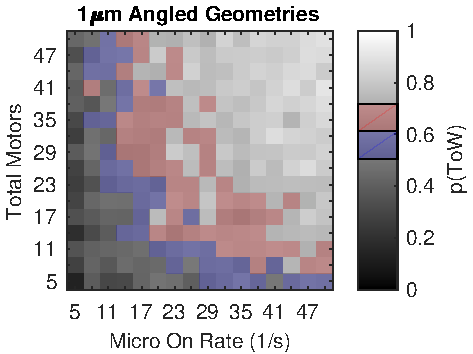
\includegraphics[width=7.75cm]{appendix1/angled1000ToW.pdf}
\\ \vspace{.5cm}
\includegraphics[width=7.75cm]{appendix1/n500ToW.pdf}
\hspace{.5cm}
\includegraphics[width=7.75cm]{appendix1/angled500ToW.pdf}
\caption[ToW probabilities for varying combinations of the unknown parameters]{ToW probabilities for varying combinations of the unknown parameters\\
ToW probabilities are shown as grey scale heat maps for a range of parameter combinations. Those which yielded ToW probabilities within the experimental 95\% confidence interval are highlighted in color. Red highlighting indicates a probability above the experimental mean, blue highlighting below. All probabilities gathered from 300 cargos. For angled geometries, 150 acute runs were grouped with 150 obtuse runs.}
\label{fig:ToW_fit}
\end{figure}

%------------------------------------------------------------------------------------------------------------------------------
\subsubsection*{Robust transport constraint}

Experimental cargos are often observed to travel along the entire length of microtubules (\SI{10}{\micro\meter} or greater). Because single motor off rates are constrained by single molecule run length experiments \cite{Block1990,Milic2014,Li2016}, we can constrain acceptable combinations of motor number and on rate by looking at simulated cargo run length. An ensemble of cargos were simulated without the crossing MT and allowed to walk until either all motors detached from the MT or a motor head passed a point \SI{10}{\micro\meter} from where the cargo started. Results are shown in figure \ref{fig:run_length_fit}. In experiments, roughly half of cargos were observed to travel the entire length of the MT.

\begin{figure}
\centering
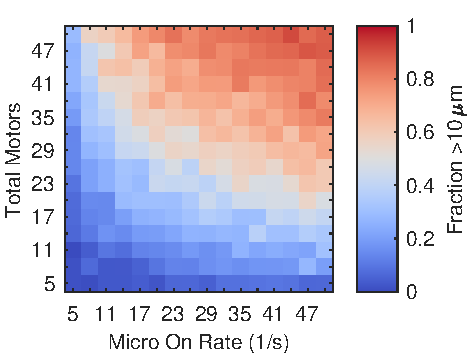
\includegraphics[width=7.75cm]{appendix1/10micronHeatmap.pdf}
\hspace{.5cm}
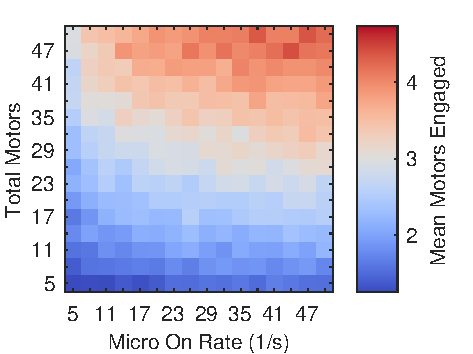
\includegraphics[width=7.75cm]{appendix1/n_ss}
\caption[Experimental observations inform selection of unknown parameters]{Experimental observations inform selection of unknown parameters \\
\textit{Left}: Fraction of cargos that travelled more than 10 microns are shown as a heat map for a range of parameter combinations. Fractions determined by simulation of 300 cargos. \\
\textit{Right}: Mean number of motors engaged on the MT at steady state is shown as a heat map for a range of parameter combinations. Values represent mean over 200 cargos. The number of motors engaged was assessed \SI{1.5}{\second} after the run began for each cargo. This time was long enough for cargos of all parameter combinations to reach steady state.}
\label{fig:run_length_fit}
\end{figure}

%------------------------------------------------------------------------------------------------------------------------------
\subsubsection*{Force constraint}

In experiments, force production of cargos was limited by the strength of the optical traps securing the bead handles. If generated forces were large enough, the forward bead handle was pulled out of its optical trap. Data for these cargos was discarded. The maximum force the bead handles could withstand was about \SI{7}{\pico\newton}, greater than the single motor stall force but less than the maximal stall force of two motors\added[id=MB,remark={Should cite the supplemental figure on this}]{}. Because experimental cargos often do not stall and geometric effects tend to keep all motors from exerting their maximal force on the bead handle at once, we expect there to be 2-3 motors exerting force on the bead handle.

Because simulated MTs are not dynamic, average or maximal simulated forces do not necessarily correspond to those one would expect to see experimentally. Therefore we investigate the number of motors simultaneously engaged on the MT at steady state, which estimates an upper limit for the number of motors simultaneously producing force.

To find the number of motors engaged on the MT, we simulate cargos walking along the primary MT without interference from a crossing MT. First, we simulate an ensemble of cargos and examine the average number of motors engaged over the ensemble as time progresses. After an initial transient, there is a period of time where neither the number of engaged motors nor the standard deviation thereof changes much. We call the average number of engaged motors during this time the steady state number. A survey of parameter combinations revealed that \SI{1.5}{\second} was long enough for cargos to come to steady state. Then, we check the average number of engaged motors at steady state for many parameter combinations. The results are shown in figure \ref{fig:run_length_fit}.

%------------------------------------------------------------------------------------------------------------------------------
\subsubsection*{Parameter selection}


A survey of figures \ref{fig:ToW_fit} and \ref{fig:run_length_fit} reveals that only parameter combinations with high numbers of total motors and low on rate fit the ToW probability and also match estimated run length and number of engaged motors. A manual search of parameter combinations in this region yielded $N=30$, $\kon^\text{micro}=\SI{10}{\per\second}$ as the best fit.

%%%%%%%%%%%%%%%%%%%%%%%%%%%%%%%%%%%%%%%%%%%%%%%%%
\section{Model Results} \label{sec:results}

Cargo trajectories were simulated forward in time as described in sections \ref{description} and \ref{sec:simulation}. Simulations were performed using the parameter values listed in table \ref{tab:params}. All parameter values used except microscopic on rate and total number of motors on the cargo are established in the literature or set by the experiment. Section \ref{param_fit} details how values for the unknown parameters were fit.

An ensemble of trajectories was simulated for a given geometry. Trajectories were categorized as described below, and probabilities of ToW and switching were derived. As shown in figure \ref{fig:trajectories}, the general behavior of simulated cargos was the same as experimental ones.

%**************************************************************************************************************
\subsection{Categorization of trajectories} \label{sec:rules}

Simulated trajectories were categorized using rules intended to emulate experimentally observed markers. Simulations began with the cargo outside of the ToW zone (section \ref{sec:ToW} and figure \ref{fig:heuristic}) and ended one of three ways: by the cargo detaching from the MT, by the cargo leaving the ToW zone on the primary MT, or by the cargo leaving the ToW zone on the crossing MT. The latter two cases were categorized as passes and switches, respectively. If the cargo detached from the primary MT before going by the intersection point, the run was discarded. If the cargo passed the intersection on the primary MT, but detached before leaving the ToW zone, the run was counted as a pass. Similarly, if the cargo was walking on the crossing MT but detached before leaving the ToW zone, the run was counted as a switch. Experimental runs were categorized using the same criteria.

Simulated cargos were marked as undergoing ToW when motors were attached to both MTs simultaneously for more than \SI{.25}{\second}. This time was selected as the minimum time in which a ToW would be detectable experimentally, given the camera frame rate. ToW time was measured as the total time during which motors were attached to both MTs and average values during ToW were accumulated during this period.

\begin{figure}
\centering
\includegraphics[width=6.5in]{appendix1/snapshots}
\caption[Snapshots from simulated cargo trajectories]{Snapshots from simulated cargo trajectories\\
During a simulation run, cargos begin outside the ToW zone with a single motor attached to the MT. Motors step stochastically, moving the cargo along the MT (\textit{left}). The cargo diffuses translationally as well as rotationally. When the cargo encounters the crossing MT, motors may bind and induce a ToW with $p(\text{ToW})$ (\textit{center,top}) or the cargo may go by the MT without any motors binding(\textit{center,bottom}). Cargos which do not ToW always pass. ToWs may end in the primary MT motor team becoming detached, resulting in a switch, with probability $p(\text{switch|ToW})$ (\textit{right,top}). Otherwise, the motor team on the crossing MT detaches, resulting in a pass (\textit{right,bottom}). To switch, a cargo must undergo ToW, then the crossing MT team must win the ToW. Therefore, the overall probability of switching $p(\text{switch})$ in given by $p(\text{ToW}) \times p(\text{switch|ToW})$.}
\label{fig:trajectories}
\end{figure}

%**************************************************************************************************************
\subsection{Encounter outcome dependance on MT geometry}

Ensembles of trajectories were simulated for varying separations and angles between the MTs. MT separations were varied from \SI{0}{\micro\meter} to \SI{1}{\micro\meter}, corresponding to 0 to 1 times the cargo diameter. Angles between the MTs were varied from nearly parallel to nearly anti-parallel. Figure \ref{fig:fractions} shows the resulting ToW and switch probabilities, along with the conditional probability of switching, given the cargo underwent ToW.

\begin{figure}
\centering
\includegraphics[width=6.5in]{appendix1/probs}
\caption[Probabilities of ToW and switching given ToW combine to explain switch probability]{Probabilities of ToW and switching given ToW combine to explain switch probability\\
\textit{A}: ToW probability as a function of the angle between the MTs is shown for separation distances corresponding to 0, 1/4, 1/2, 3/4 and 1 times the cargo diameter. Simulated data shown with thin bars representing standard error. Curves represent quadratic fits to simulated data for all but \SI{.25}{\micro\meter} separation distance, which is fit to a quadratic with an overlaid gaussian. Experimental data shown with think bars representing 95\% confidence interval.\\
\textit{B}: Conditional probability of switching, given the cargo undergoes ToW. Data represented as in \textit{A}.\\
\textit{C}: Overall switch probability. Data represented as in \textit{A}}
\label{fig:fractions}
\end{figure}

%**************************************************************************************************************
\subsection{Explanation of ToW probability} \label{sec:ToW}

In agreement with intuition, ToW probability increases with the distance the cargo must travel while able to reach both MTs simultaneously, which we call the ToW zone, denoted $x_\text{ToW}$. The extent of the ToW zone was calculated from geometry diagrammed in figure \ref{fig:heuristic}, and is given by
\begin{multline} \label{eq:ToW_zone}
x_\text{ToW}=2\frac{ \sqrt{4 (L+R+R_{MT})^2-\left( (\xmt^1-\xmt^2)\cdot \hat{z} \right)^2} }{\norm{\dmt^1 \cross \dmt^2}} \\
= 2\frac{ \sqrt{4 (L+R+R_{MT})^2-\left( \text{separation distance} \right)^2} }{\sin(\text{MT angle})}.
\end{multline}
The probability a cargo will undergo ToW can then be understood as a competition between the rate at which the cargo binds to the crossing MT, which happens at a rate which we denote $\kon^\text{macro}$, and the rate it leaves the ToW zone, which happens at a rate given by the cargo velocity (equal to the maximum single motor velocity $v$) divided by the ToW zone length. Thus,
\begin{equation} \label{eq:rate_war}
p(\text{ToW})=\frac{ \kon^\text{macro}}{\kon^\text{macro} +  \frac{v}{x_\text{ToW}}}.
\end{equation}
The rate at which the cargo attaches to the crossing MT, $\kon^\text{macro}$, is in general a complex function of geometry as well as motor and cargo parameters. However, for this heuristic analysis we assume it is constant across different geometries. If we fit the macro on rate to the experimental data on ToW probability, we recover the qualitative features of the full simulation result as shown in figure \ref{fig:heuristic}.

\begin{figure}
\centering
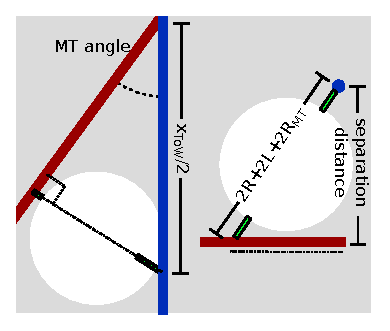
\includegraphics[width=6cm]{appendix1/ToWzone}
\includegraphics[width=10cm]{appendix1/heuristicSIM.pdf}
\caption[A heuristic model matches qualitative features of ToW probability]{A heuristic model matches qualitative features of ToW probability\\
\textit{Left}: Diagram of the ToW zone. The ToW zone is defined as the distance along the primary MT in which the cargo can reach the crossing MT. Its length was calculated geometrically and is given by equation \ref{eq:ToW_zone}. Primary MT is shown in blue, crossing MT in red, motors in green and cargo in white. \\
\textit{Right}: Solutions to the heuristic model for ToW probability. The heuristic model poses the probability of undergoing ToW as the the probability of the cargo binding (with constant binding rate) to the crossing MT before leaving the ToW zone and is given in equation \ref{eq:rate_war}. Experimental probabilities are shown with error bars representing 95\% confidence interval. Bars for data at \SI{.5}{\micro\meter} shifted slightly to aid the eye. Solutions plotted with $\kon^\text{macro}$ set to \SI{1}{\per\second}. 
}
\label{fig:heuristic}
\end{figure}

%------------------------------------------------------------------------------------------------------------------------------
\subsubsection*{Steric effects strongly influence ToW probabilities in \SI{0}{\micro\meter} and \SI{.25}{\micro\meter} geometries}

A comparison of figures \ref{fig:heuristic} and \ref{fig:fractions}A reveals that the heuristic model captures the features of ToW probability for MT separations \SI{.5}{\micro\meter} and greater very well. However, it fails to reproduce features of the simulated data at \SI{.25}{\micro\meter} and \SI{0}{\micro\meter}. This failure shows that the peak in ToW probability near the normal for \SI{.25}{\micro\meter} separation and the overall high ToW probability at \SI{0}{\micro\meter} must result from effects not considered in the heuristic model. As discussed in the main text, steric interactions play a large role.

%**************************************************************************************************************
\subsection{Explanation of conditional probability of switching given ToW}

The complex dependence of conditional probability of switching on geometry is not intuitive and warrants further investigation. To this end, we show the mean number of motors engaged on each MT during ToW, the mean forces exerted on the motor teams during ToW, the ToW time, and how each of these depends on the MT geometry in figure \ref{fig:ToW_forces}. Below we explain the behavior of the simulated conditional probability of switching on geometry using these results.

\begin{figure}
\centering
\includegraphics[width=6.5in]{appendix1/forces}
\caption[Numbers engaged, forces and ToW times explain conditional probability of switching]{Numbers engaged, forces and ToW times explain conditional probability of switching\\
\textit{A}: Mean number of motors engaged during ToW for primary and crossing MT teams. The numbers are shown as a function of MT angle. Below, the ratio of mean motors engaged on the crossing MT to the primary MT is shown. Separation distances are colored as described in the legend in the top panel of \textit{A}. Error bars represent standard error of the mean. \\
\textit{B}: Mean force experienced by the motor teams on the primary and crossing MTs during ToW. Forces are shown as a function of angle. Below, the ratio of the forces on the crossing MT team to the forces on the primary MT team is displayed. Data represented as in \textit{A}.\\
\textit{C}: Mean steric force exerted by the primary and crossing MTs during ToW. Forces shown as a function of angle and represented as in \textit{A}.
\textit{D}: Mean ToW time as a function of angle between the MTs. ToW time is the total time motors are engaged on both MTs. Data represented as in \textit{A}.}
\label{fig:ToW_forces}
\end{figure}

%------------------------------------------------------------------------------------------------------------------------------
\subsubsection*{\SI{1}{\micro\meter} near-normal geometries}

At \SI{1}{\micro\meter} separation distance, the cargo can not sterically interact with both MTs at once. Since forces exerted by the MTs are minimal (figure \ref{fig:ToW_forces}C), motor teams in these ToWs pull directly on each other, as evidenced by high forces on the motor teams and a ratio near 1, shown in figure \ref{fig:ToW_forces}B. Furthermore, ToW times are short (figure \ref{fig:ToW_forces}D), meaning the crossing MT team often only gets one chance to cause a switch. One might expect, then, that since the ratio of crossing MT to primary MT motor number is $\approx .7$ (figure \ref{fig:ToW_forces}A), switches would happen about 30\% of the time. However, a ToW between motor teams of different numbers is not directly determined by motor numbers. The slow increase of unbinding rate above stall gives the smaller team a significant chance to win the ToW, leading to an overall probability of switching higher than 30\%, but still below 50\%.

%------------------------------------------------------------------------------------------------------------------------------
\subsubsection*{\SI{1}{\micro\meter} acute geometries}

Conditional probabilities of switching at \SI{1}{\micro\meter} are slightly higher for acute geometries  than they are near the normal. As in the latter, motors pull directly on each other during ToWs, evidenced by high forces in figure \ref{fig:ToW_forces}B. However, an asymmetry exists between a ToW won by the crossing MT motor team and the primary MT motor team in acute geometries. When the primary MT motor team wins a ToW, the cargo continues on through the ToW zone (which is longer for more acute geometries, see equation \ref{eq:ToW_zone}). During this time motors may again bind to the crossing MT, giving another chance for a switch. Evidence of this effect can be seen in the longer ToW times shown in figure \ref{fig:ToW_forces}D. However, when the crossing MT team wins a ToW, the cargo is likely to diffuse down and away from the primary MT and avoid rebinding. This effect drives switching up slightly for acute geometries compared to near-normal.

%------------------------------------------------------------------------------------------------------------------------------
\subsubsection*{\SI{1}{\micro\meter} obtuse}

Unlike in near-normal and acute geometries at \SI{1}{\micro\meter}, motors in obtuse geometries feel low average forces, as shown in figure \ref{fig:ToW_forces}B. ToW times are long, as seen in figure \ref{fig:ToW_forces}D, because MT alignment is close to parallel and motors walk in nearly the same direction. Motors do not feel significant load until the cargo has moved far enough from the intersection that the distance from MT to MT is greater than twice the bead diameter. These long periods of walking under low force turn the ToW into a competition of processivity as much as force. While a smaller motor team can compete against a larger motor team in a force competition, processivity grows quickly with motor number, so larger motor teams are more likely to win a processivity competition. Because there are on average more motors on the primary MT team, the probability of switching goes down as the distance walked goes up with more obtuse angles.

%------------------------------------------------------------------------------------------------------------------------------
\subsubsection*{\SI{.5}{\micro\meter} near-normal geometries}

In \SI{.5}{\micro\meter} geometries, the cargo must hurdle up and over the crossing MT to pass. If the cargo is underneath the primary MT, the primary MT motors are loaded as they pull the cargo into the crossing MT, but the cargo cannot pass the intersection until it is out from underneath the primary MT. In near-normal geometries, the crossing MT team assists this process by pulling the cargo out toward the plus end of the crossing MT. While this is taking place, the primary MT motors continue to be loaded. This load sometimes causes primary MT motors to unbind, leading to a weaker team on average. As crossing MT motors walk, the force from the primary MT motors is shifted from the crossing MT to the crossing MT motor team. In the end, this interaction has similar dynamics to the ones described in the \SI{1}{\micro\meter} near-normal geometries, albeit with a primary MT motor team that is now weaker on average. This slightly biases the ToW toward the crossing MT team relative to \SI{1}{\micro\meter} near-normal geometries, resulting in a ToW probability near 50\%.

%------------------------------------------------------------------------------------------------------------------------------
\subsubsection*{\SI{.5}{\micro\meter} acute geometries}

Unlike in near-normal geometries at \SI{.5}{\micro\meter}, the crossing MT motors do not aid hurdling behavior in acute geometries. In fact, they impede hurdling; when the crossing MT motors engage, they act to wedge the cargo between the MTs, described as "chop-sticking" in the main text. This effect can be seen in the high forces exerted by the MTs at these geometries shown in figure \ref{fig:ToW_forces}C. Because crossing MT motors impede hurdling and the cargo must travel beyond the intersection to pass, crossing MT motors often get multiple chances to cause a switch, indicated by long ToW times in figure \ref{fig:ToW_forces}D. This leads to the conditional probability of switching rising 50\%.

%------------------------------------------------------------------------------------------------------------------------------
\subsubsection*{\SI{.5}{\micro\meter} obtuse geometries}

As in \SI{.5}{\micro\meter} near-normal geometries, crossing MT motors aid hurdling in \SI{.5}{\micro\meter} obtuse geometries. Additionally, like obtuse geometries at \SI{1}{\micro\meter} separation distance, ToW times are long (figure \ref{fig:ToW_forces}D) and forces are low (figure \ref{fig:ToW_forces}B). As described, this biases the ToW toward the larger motor team on the primary MT and results in less switching.

%------------------------------------------------------------------------------------------------------------------------------
\subsubsection*{\SI{.25}{\micro\meter} and \SI{.75}{\micro\meter} geometries}

The conditional probability of switching in \SI{.25}{\micro\meter} and \SI{.75}{\micro\meter} geometries is similar to that of \SI{.5}{\micro\meter} geometries, indicating the same mechanisms are at play. There is a significant deviation at angles near the normal in \SI{.25}{\micro\meter} geometries. At these angles, the crossing MT becomes a very effective barrier to progress of the cargo. Because the crossing MT is above the cargo equator, steric forces from the crossing MT tend to push the cargo back down, causing it to get stuck below the intersection. This effect can be seen in the high MT forces near normal in figure \ref{fig:ToW_forces}C. Stuck cargos are more likely to switch, leading to an overall high switching probability.

%------------------------------------------------------------------------------------------------------------------------------
\subsubsection*{\SI{0}{\micro\meter} near-normal geometries}

As explained in the main text, cargos may only pass two ways in \SI{0}{\micro\meter} geometries: by the cargo hurdling up and over the crossing MT, or by monkey-barring. Since cargos experience a gravitational force, they are likely to encounter the intersection below the crossing MT and not be able to hurdle. Because successful monkey-barring is a process which requires two rare events, this leads to a high probability of switching.

%------------------------------------------------------------------------------------------------------------------------------
\subsubsection*{\SI{0}{\micro\meter} acute geometries}

Because the ToW zone is longer in acute geometries than near-normal, cargos are more likely to undergo several ToW events. This is reflected in the long ToW times at acute geometries shown in figure \ref{fig:ToW_forces}D. In the opposite effect of that in \SI{.5}{\micro\meter} geometries, these longer ToWs lead to less switching in \SI{0}{\micro\meter} geometries. This is because these longer ToWs give the cargo more chances to monkey-bar and pass the intersection.

%------------------------------------------------------------------------------------------------------------------------------
\subsubsection*{\SI{0}{\micro\meter} obtuse geometries}

Conditional probability of switching falls as angles become closer to parallel for \SI{0}{\micro\meter} separation distance, and approaches 50\%. The forces on the cargo in these geometries are such that motors on the crossing MT tend to pull the cargo up and over the top of the intersection. This leads to greater ease of passing because the crossing MT no longer blocks progress of the primary MT motor team when the cargo is above the plane.

%\newpage
%
%\vspace*{2\baselineskip}
%\centerline{\textbf{\LARGE Captions for supplemental movies}}
%\vspace{4\baselineskip}
%
%\begin{itemize}[label={}]
%
%\item \textbf{Supplement Movie 1.} Intersection geometry: \SI{0.5}{\micro\meter} separation, \ang{90} angle.  MC engages in ToW, and ultimately passes. For detailed analysis of this event, see Fig. 2A,B,D. The video has been rescaled 3X for clarity.
%
%\item \textbf{Supplement Movie 2.} Intersection geometry: \SI{0.5}{\micro\meter} separation, \ang{90} angle.  MC engages in ToW, and ultimately switches. For detailed analysis of this event, see Fig. 2C. The video has been rescaled 3X for clarity.
%
%\item \textbf{Supplement Movie 3.} Intersection geometry: \SI{1}{\micro\meter} separation, \ang{90} angle.  MC engages in ToW, and ultimately switches.
%
%\item \textbf{Supplement Movie 4.} Intersection geometry: \SI{1}{\micro\meter} separation, \ang{90} angle.  MC engages in ToW and ultimately passes.
%
%\item \textbf{Supplement Movie 5.} Intersection geometry: \SI{0.5}{\micro\meter} separation, \ang{90} angle.  MC engages in ToW, "hurdles" over the crossing MT, and ultimately switches.  
%
%\item \textbf{Supplement Movie 6.} Intersection geometry: \SI{0.5}{\micro\meter} separation, \ang{90} angle.  MC engages in ToW, "hurdles" over the crossing MT, and ultimately passes. 
%
%\item \textbf{Supplement Movie 7.} Intersection geometry: \SI{0}{\micro\meter} separation, \ang{90} angle. The motors engaged on the primary MT are initially blocked. Other motors then engage the crossing MT, and the MC switches.
%
%\item \textbf{Supplement Movie 8.} Intersection geometry: \SI{0}{\micro\meter} separation, \ang{90} angle. MC ToWs and then and ultimately passes via "monkey-barring."
%
%\item \textbf{Supplement Movie 9.} Intersection geometry: \SI{0}{\micro\meter} separation, \ang{90} angle. Simulated viscosity: \SI{1}{\pascal\second} (1000x as viscous as water).  MC ToWs and then and ultimately switches.
%
%\item \textbf{Supplement Movie 10.} Intersection geometry: \SI{0.5}{\micro\meter} separation, acute angle. When the MC engages in a ToW, the ability to hurdle is suppressed ("chop-sticking").  The MC ultimately switches.  
%
%\end{itemize}
%
%\newpage
%
%\newrefcontext[labelprefix=S]
%\printbibliography
%
%\end{document}
